\documentclass[tikz]{standalone}
\usepackage{tikz}
\usetikzlibrary{calc}
\usetikzlibrary{positioning}
\usetikzlibrary{fit}
\usetikzlibrary{backgrounds}

\definecolor{lightGreen}{HTML}{d5e8d4}
\definecolor{lightYellow}{HTML}{fff2cc}
\definecolor{lightGray}{HTML}{f5f5f5}
\definecolor{lightRed}{HTML}{ff9999}
\definecolor{lightBlue}{HTML}{d5e5fc}
\definecolor{lightCyan}{HTML}{a7dfe3}
\pgfdeclarelayer{main_bg}
\pgfdeclarelayer{back_bg}
\pgfsetlayers{back_bg,main_bg,main}

\newcommand{\metarect}[7]{
    \begin{scope}
        \node (#1) [rectangle, draw, text width=\rectWidth, minimum width=\rectWidth, minimum height=\rectHeight, #7] {};
        \node (#1_upper) [rectangle, draw, fill=#6, text width=\rectWidth, minimum width=\rectWidth, minimum height=\rectHeight*0.5, below=0.0pt of #1.north, anchor=north] {#2};
        \node (#1_middle) [rectangle, draw, fill=white, font=\tiny, text width=\rectWidth, minimum width=\rectWidth, minimum height=\rectHeight*0.25, below=-\the\pgflinewidth of #1_upper] {#3};
        \node (#1_bleft) [rectangle, draw, fill=white, font=\tiny, text width=\rectWidth*0.35, minimum width=\rectWidth*0.35, minimum height=\rectHeight*0.25, below=-\the\pgflinewidth of #1_middle.south west, anchor=north west] {#4};
        \node (#1_bright) [rectangle, draw, fill=white, font=\tiny, text width=\rectWidth*0.65, minimum width=\rectWidth*0.65, minimum height=\rectHeight*0.25, right=-\the\pgflinewidth of #1_bleft] {#5};
    \end{scope}
}

\begin{document}
    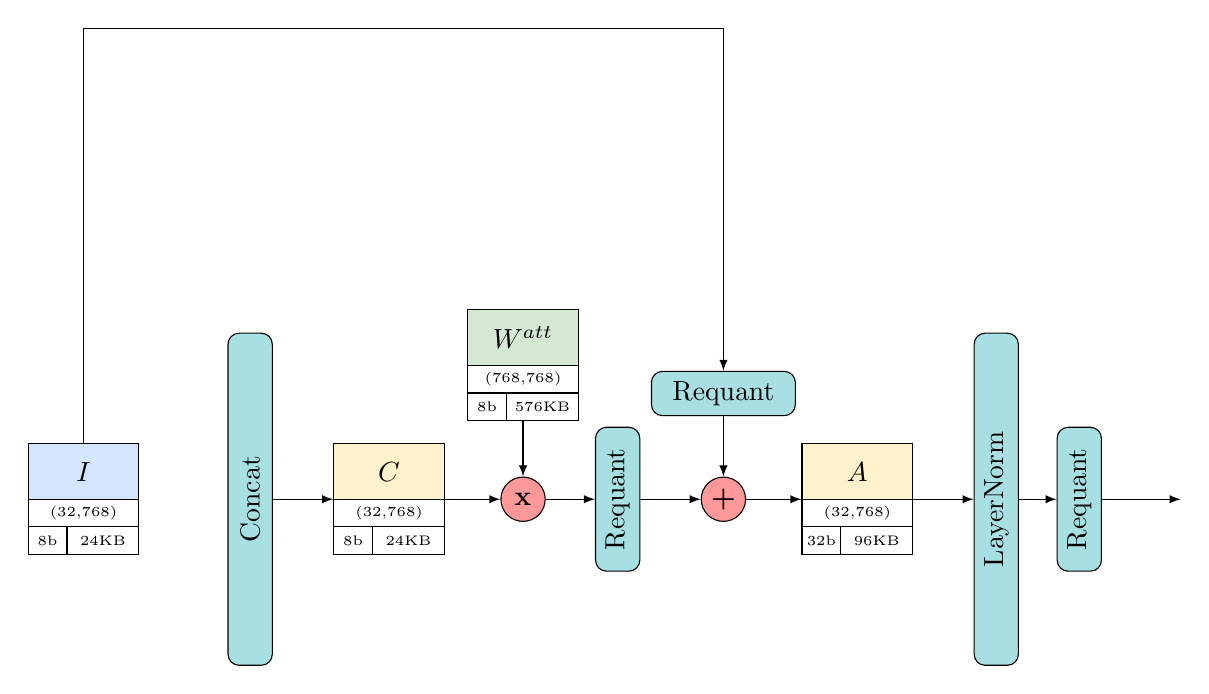
\begin{tikzpicture}[inner sep=0.0 pt, align=center]
    \pgfmathsetmacro{\rectWidth}{40}
    \pgfmathsetmacro{\rectHeight}{40}

    \metarect{layer_input}{$I$}{(32,768)}{8b}{24KB}{lightBlue}{}

    \pgfmathsetmacro{\multSize}{16 pt}

    \node [draw, fill=lightCyan, rounded corners, minimum width=\rectHeight*3, minimum height=\rectWidth*0.4, rotate=90, right=\rectWidth*1pt of layer_input, anchor=center] (concat) {Concat};

    \metarect{C}{$C$}{(32,768)}{8b}{24KB}{lightYellow}{right=\rectWidth*0.75pt of concat.center}
    \node [draw, circle, fill=lightRed, minimum size=\multSize, right=\rectWidth*0.5pt of C] (multAtt) {\textbf{x}};
    \metarect{weight_att}{$W^{att}$}{(768,768)}{8b}{576KB}{lightGreen}{above=\rectHeight*0.5pt of multAtt}
    \node [draw, fill=lightCyan, rounded corners, minimum width=\rectHeight*1.3, minimum height=\rectWidth*0.4, rotate=90, right=\rectWidth*0.65pt of multAtt, anchor=center] (C_W_req) {Requant};
    \node [draw, circle, fill=lightRed, minimum size=\multSize, right=\rectWidth*0.75pt of C_W_req.center] (addAtt) {\textbf{+}};
    \node [draw, fill=lightCyan, rounded corners, minimum width=\rectHeight*1.3, minimum height=\rectWidth*0.4, above=\rectWidth*0.75pt of addAtt, anchor=center] (I_req) {Requant};
    \metarect{A}{$A$}{(32,768)}{32b}{96KB}{lightYellow}{right=\rectWidth*0.5pt of addAtt}

    \draw [-latex] (concat.south) -- (C.west);
    \draw [-latex] (C.east) -- (multAtt.west);
    \draw [-latex] (weight_att.south) -- (multAtt.north);
    \draw [-latex] (multAtt.east) -- (C_W_req.north);
    \draw [-latex] (C_W_req.south) -- (addAtt.west);
    \draw [-latex] (addAtt.east) -- (A.west);

    \draw [-latex] (layer_input.north) -- ++(0pt,\rectHeight*3.75pt) -| (I_req.north);
    \draw [-latex] (I_req.south) -- (addAtt.north);

    \node [draw, fill=lightCyan, rounded corners, minimum width=\rectHeight*3, minimum height=\rectWidth*0.4, rotate=90, right=\rectWidth*0.75pt of A, anchor=center] (ln1) {LayerNorm};
    \node [draw, fill=lightCyan, rounded corners, minimum width=\rectHeight*1.3, minimum height=\rectWidth*0.4, rotate=90, right=\rectWidth*0.75pt of ln1.center, anchor=center] (A_out_req) {Requant};

    \draw [-latex] (A.east) -- (ln1.north);
    \draw [-latex] (ln1.south) -- (A_out_req.north);
    \draw [-latex] (A_out_req.south) -- ++(1,0);

%    \begin{pgfonlayer}{main_bg}
%        % fill=red!3
%        \node (all) [draw, rectangle, inner sep=40pt, fit=(layer_input)(weight_Q)(weight_K)(weight_V)(mixQ32b)(mixV32b)(Ci8b)(O_tilde)] {};
%    \end{pgfonlayer}
    \end{tikzpicture}

\end{document}
